The data that is obtained from the sensors generates a continuous data stream for every sensor. A good feature representation of the data is required so that the LDA model can be applied. First the sensors are divided into five fields and all the data that is generated from one field is combined into one data stream. In this way the data is reduced to five dimensions. 
The continuous data stream cannot be used as input for the LDA model. Therefore, like it is done in the work of Farrahi \cite{farrahi2008daily}, the data of one day is divided into time-slices of length $l$. For a chosen length of the time-slices $l$ in minutes, the number of time-slices for one day can then be calculated with $n=1440/l$ (there are 1440 minutes per day) So for example if the length of the time-slices is $l=30$ min. then the number of time-slices on one day is $n=48$. A day starts and ends at 3 a.m. in the morning. In this way the chance to cut between activities is reduced. It still can occur that a person goes to bed late or that he needs to visit the toilet. For now this fact is left out in the part of modeling.\\

For every field  the number of activations is counted in each time-slice. An sensor activation is defined as the change of the signal from zero  to one. The duration of an active signal is not taken into account. In this way a door that accidentally is left open will not generate a high value, which will otherwise disturb the data. Every field then forms a dimension of the observations $o_n$. An observation can be seen as an artificial word. In figure \ref{fig:FeatEx} an example on how the data is translated into a vector representation is given for one time-slice.\\

\begin{figure}[h]
\centering
\begin{minipage}{0.55\linewidth}
\centering
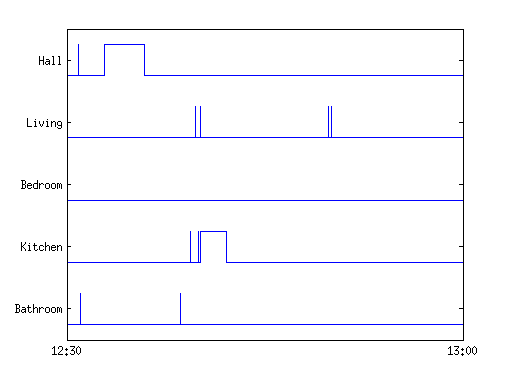
\includegraphics[width=\textwidth]{Pictures/FeatExample.png}
\end{minipage}
\begin{minipage}{0.35\linewidth}
\centering
\begin{equation*}
\vec{o}_n = 
 \begin{bmatrix} 
 o_{Hall}\\
 o_{Living}\\
 o_{Bedroom}\\
 o_{Kitchen}\\
 o_{Bathroom}\\
 o_{time}
 \end{bmatrix}
 =
  \begin{bmatrix} 
 2\\
 4\\
 0\\
 3\\
 2\\
 t
 \end{bmatrix}
\end{equation*}
\end{minipage}
\caption{Vector representation of the data. The data of the sensors is shown in the left image. It is translated in the vector shown on the right-hand side.}
\label{fig:FeatEx}
\end{figure}

The last dimension of the observation $\vec{o}_n$ represents the time value of a time-slice. There are two different ways how the time dimension is added to the observations. In the fine-grain representation the time value becomes the number of the time-slice. In figure \ref{fig:FeatEx} the 30 minutes time interval $[12:30,13:00]$ is the 20th time-slice on a day that starts at 3 a.m. In this way the observation will become $\vec{o}_n=\{2,4,0,3,2,20\}$. In the coarse-grain representation, which is also used in the work Farrahi et al. \cite{farrahi2008daily} and Castanedo et al. \cite{EXSY:EXSY12033}, the 24 hours of a day are divided into the five time intervals $\{ 3am - 8am, 8am - 1pm, 1pm - 18pm, 18pm - 23pm, 23pm - 3am  \}$. In this way the observation of figure \ref{fig:FeatEx} will become $o_n=\{2,4,0,3,2,2\}$.\\

The data sets that are used in this thesis contain a minimum of 68 and a maximum of 142 days of data. With the chosen feature representation there are a lot of possible observations, which are not contained in the data sets. In the data the maximum value of 28 is observed in one field, when the number of time-slices per day is $n=48$. This is an extreme value and occurs not that often in the data. If the maximum value for each field is assumed to be 15 and the time-dimension is fine grain, there are approximately 36 million ($15^5*48$) possible observations that can be made. As a comparison: In the work of Farrahi \cite{farrahi2008daily} only 512 ($4^3*8$) different observations are possible and 2856 days of data for 68 people is available.\\
In table \ref{tab:features} an overview is given how many unique words are actual observed for the different houses and how many words are totally observed ($48*\text{\# of days}$). One can see that the number of unique observations scales with the number of days available for each house. This also shows that in the data a lot of possible observations are not included. In figure \ref{fig:occurence} the occurrence for each unique word is shown on the y-axis for the data of house number one. The words that occur the most have zero values for the first five dimensions and different values for the sixth dimension (time). Most other unique words only occur once. Therefore applying the LDA model to this simple BOW representation is not feasible.\\


\begin{table}
\caption{}
 \centering
 \begin{tabular}{l c c c c c}
  HouseNr & 1 & 2 & 3 & 4 & 5\\
  \hline
  \# of days & 142 & 98 & 89 & 63 & 73 \\
  observations & 6816 & 4704 & 4272 & 3024 & 3504 \\
  unique observations & 3017 & 2110 & 2288 & 1269 & 1490\\
 \end{tabular}
 \label{tab:features}
\end{table}



\begin{figure}[h]
 \centering
 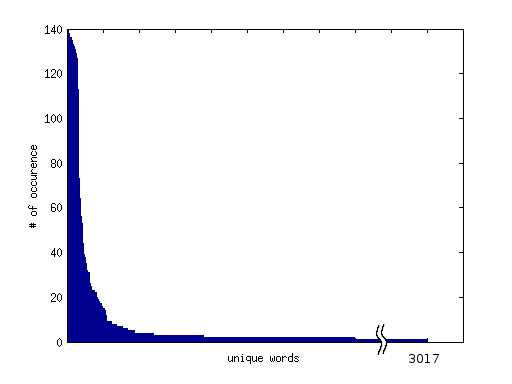
\includegraphics[width=0.9\textwidth]{Pictures/Occ.png}
 \caption{Occurrence of unique observation for house number one.}
 \label{fig:occurence}
\end{figure}


In figure \ref{fig:FieldDistr} for each dimension of the observations a histogram is created of the activation values in the set of unique observations. For the first five dimension, which corresponds to the sensor values, small values are more probable to appear in the vocabulary. The found distribution is comparable to a Poisson-distribution. The sixth dimension, which corresponds to the time, shows that there are more unique observations that have a time value between 15 and 43. This makes sense because there is more activity during daytime which leads to more variate observations in this time period.\\


\begin{figure}[h]
 \centering
 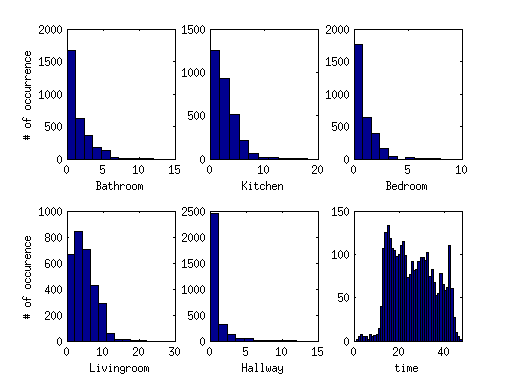
\includegraphics[width=0.9\textwidth]{Pictures/OccField2.png}
 \caption{Occurrence of observation per field/dimension in the set of unique words for house number one.}
 \label{fig:FieldDistr}
\end{figure}

The given feature representation, with the two variation of the time dimensions, fine grain and coarse grain, are used in the following chapters. There are much more possibilities to describe the features, which is further explained in the future work (see chapter \ref{chapter:conclusions}).
